\documentclass{article}
\usepackage[letterpaper,top=2cm,bottom=2cm,left=3cm,right=3cm,marginparwidth=1.75cm]{geometry}
\usepackage[russian]{babel}
\usepackage{amsmath}
\usepackage{graphicx}
\usepackage[utf8]{inputenc}
\usepackage[colorlinks=true, allcolors=blue]{hyperref}
\usepackage[pdf]{graphviz}
\graphicspath{ {./static/} }
\usepackage{ucs} 
\usepackage[T1]{fontenc}


% Listing % 
\usepackage{listings}
\usepackage{color}
\usepackage{minted}

\definecolor{dkgreen}{rgb}{0,0.8,0}
\definecolor{gray}{rgb}{0.5,0.5,0.5}
\definecolor{mauve}{rgb}{0.58,0,0.82}



% Graphics  % 

\usepackage{graphicx}
\graphicspath{ {./static/} }


\title{ТМВ Домашнее задание №3}
\author{А-13б-19 Головин Антон}
\date{29 мая 2022}


\begin{document}
\maketitle


%%%%%%%%%%%%%%%%%%%%%%%% Упражнение 1 %%%%%%%%%%%%%%%%%%%%%%%%


\section*{2. Машины Тьюринга}

\subsection*{2.1 Операции с языками и символами}

Реализуйте машины Тьюринга, которые позволяют выполнять следующие операции:
\begin{enumerate}

    %%%%%%%%%%%%%%% 1 %%%%%%%%%%%%%%%
    \item \textbf{Сложение двух унарных чисел (1 балл)}
    
        Алгоритм:
        \begin{itemize}
            \item Движемся вправо, пока не встретили '+'.
            \item Заменяем '+' на 1 и движемся к хвосту.
            \item Находим крайнюю единицу и удаляем её.
            \item Движемся к голове.
        \end{itemize}
        
        
        \begin{minted}[]{yaml}
            # 2_1_1.yaml
            input: '111+1'
            blank: ' '
            start state: right
            table:
              right:
                1: R
                '+': {write: '1', R: tail}
              tail:
                1: R
                ' ': {L: del_and_return}
              del_and_return:
                1: {write: ' ', L: return}
              return:
                1: L
                ' ': {R: done}
              done:
        \end{minted}
        
        \begin{center}
            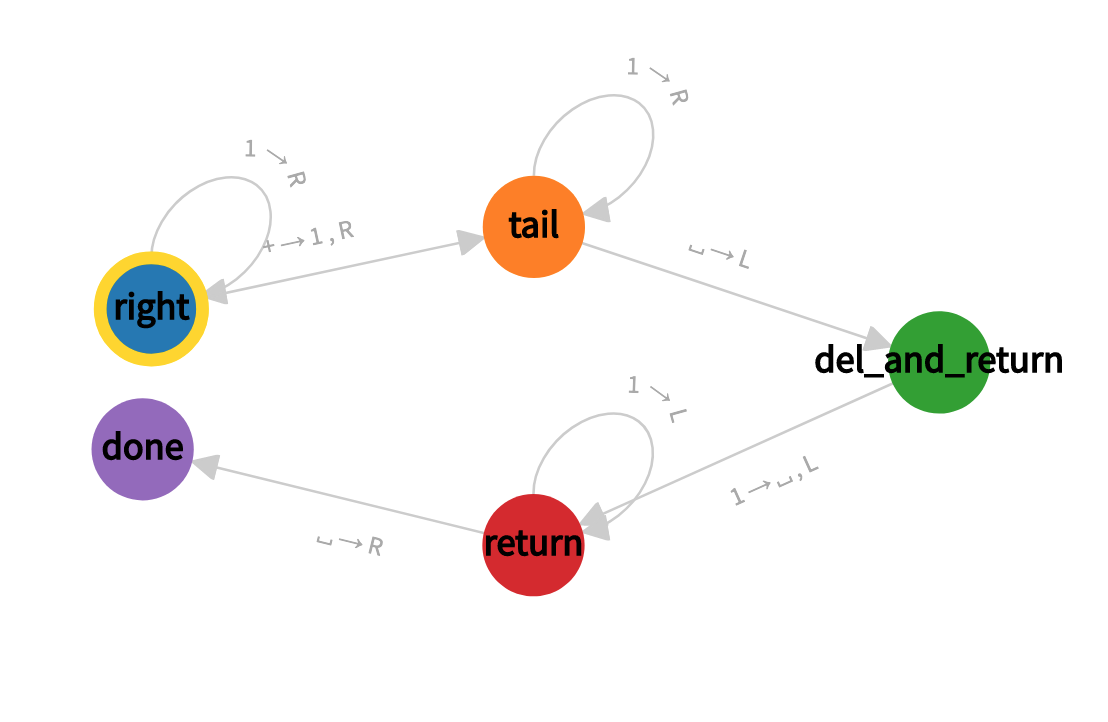
\includegraphics[width=0.6\textwidth]{2_1_1.png} \\
        \end{center}
    %%%%%%%%%%%%%%%%%%%%%%%%%%%%%%%%%
    
    %%%%%%%%%%%%%%% 2 %%%%%%%%%%%%%%%
    \item \textbf{Умножение унарных чисел (1 балл)}
    
        Копируем за знак '=' единицы первого множителя столько раз, сколько единиц во втором.
        
        Алгоритм:
        \begin{itemize}
            
            \item Двигаемся вправо и находим '*', потом помечаем первую найденную единицу второго множителя крестиком 'x'.
            \item Движемся влево и начинаем копирование - все единицы первого множителя помечаем крестиком и записываем после знака '='.
            \item Пока мы не встретили '$\lambda$' в начале, продолжам копирование.
            \item Встретили '$\lambda$' - восстанавливаем единицы первого множителя (пока не встретим '*').
            \item Повторяем шаги (помечаем 'x' единицы второго множителя, пока это возможно).
            \item Когда не осталось единиц, умножение завершено, восстанавливаем все единицы. 
        \end{itemize}

        \begin{minted}[]{yaml}
            # 2_1_2.yaml
            input: '111*11'
            blank: ' '
            start state: check-correct
            
            
            table:
            
              # проверка случаев 1* и *1
              check-correct:
                1: {R: check-star}
                '*': {L: check-empty}
              check-star:
                1: R
                '*': {R: check-empty}
              check-empty:
                ' ': {R: done}
                1: {L: go-start}
              
              
              go-start:
                [1, '*', '=']: {L: go-start}
                ' ': {R: preload}
              
              preload:              # добавляем = 
                [1, '*']: R
                ' ': {write: '=', R: λ-end}
              λ-end:                # добавляем λ в конец
                ' ': {write: 'λ', L: λ-start}
                [1, '=', '*']: L
              λ-start:              # добавляем λ в начало
                ' ': {write: 'λ', R: start}
                ['λ', '=', '*', 1]: L
                
                
              start:              
                1: R
                ['x', '*']: {R: process-second}
                
              process-second:
                'x': R
                1: {write: 'x', L: go-first}
                '=': {L: clear-λ-start}   # копировать нечего
              
              remain-ones:        # проверяем, нужно ли нам копировать снова
                [1, '=']: {L: go-first}
                
              
              go-first:
                ['x', '*']: L
                1: {write: 'x', R: copy}
                'λ': {R: restore} 
              
              restore:            # очередное копирование завершено, восстанавливаем 1
                'x': {write: 1, R: restore}
                '*': {R: start}
                
              copy:
                [1, '*', 'x', '=']: R
                'λ': {write: 1, R: go-end}
              
              go-end:
                ' ': {write: 'λ', L: go-second}
              
              go-second:
                [1, 'x', '=']: L
                '*': {L: go-first}
            
              clear-λ-start: 
                'x': {write: 1, L: clear-λ-start}
                [1, '*']: L
                'λ': {write: ' ', R: clear-λ-end}
                
              clear-λ-end:
                [1, '*', 'x', '=']: R
                'λ': {write: ' ', L: finish}
                
              finish:
                  [1, '*', 'x', '=']:  L
                  ' ': {R: done}
                  
              done:
        \end{minted}
        \begin{center}
            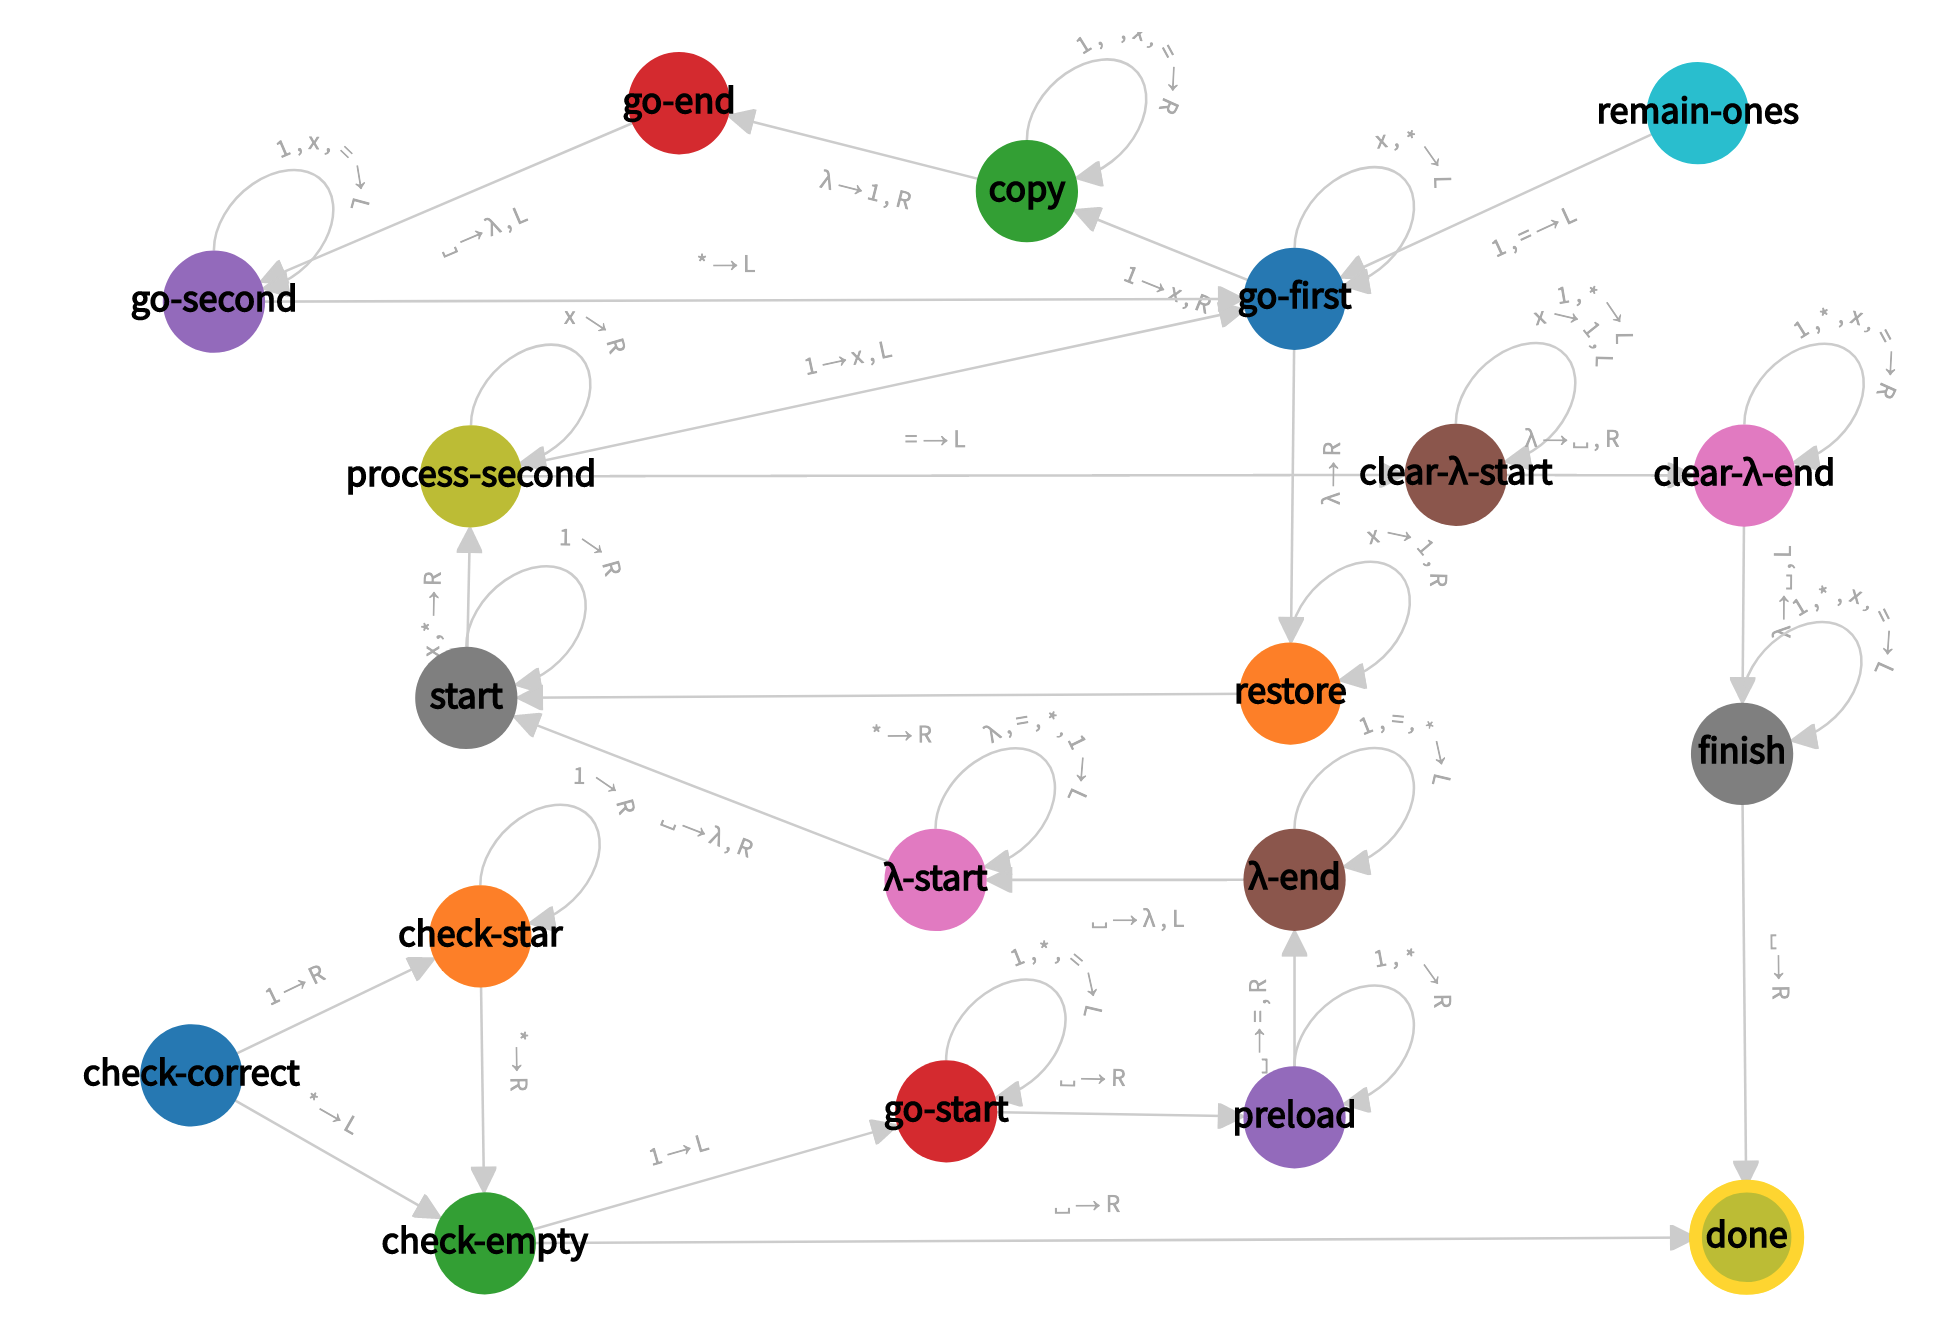
\includegraphics[width=\textwidth]{2_1_2.png} \\
        \end{center}
    
\end{enumerate}


\subsection*{2.2 Операции с языками и символами}
Реализуйте машины Тьюринга, которые позволяют выполнять следующие операции:

\begin{enumerate}

    %%%%%%%%%%%%%%% 1 %%%%%%%%%%%%%%%
    \item Принадлежность к языку $L = \{ 0^n1^n2^n \}, n \ge 0$ (0.5 балла)
    
        Алгоритм:
        \begin{itemize}
            \item Все первые вхождения 0, 1, 2 заменяем на 'x'. Возвращаемся в начало.
            \item Повторяем шаг выше, пока слово не будет заменено на все 'x' (иначе слово не принадлежит языку).
            \item 1 - слов принадлежит языку, 0 - нет
            \item По усновию $n$ может быть равно 0, поэтому пустое слово тоже принадлежит языку. 
        \end{itemize}
        
        \begin{minted}[]{yaml}
            # 2_2_1.yaml
            input: '012012'
            blank: ' '
            start state: start
            
            
            table:
              start:
                ' ': {L: ok}    # слово принадлежит языку
                0: {write: 'x', R: go-one} 
                [1, 2]: {R: not-ok}
                'x': R            # новый проход
              
              go-one:
                [0, 'x']: R    
                1: {write: 'x', R: go-two} 
                [2, ' ']: {L: not-ok}
              
              go-two:
                ' ': {L: not-ok}
                [1, 'x']: R
                2: {write: 'x', L: go-start}
            
              
              go-start:
                ' ': {R: start}
                [0, 1, 2, 'x']: L 
                
              ok:
                ' ': {write: 1, L: done}
                'x': {write: ' ', L}
              
              not-ok:
                ' ': {L: del}
                [0, 1, 2, 'x']: R
              
              del:
                ' ': {write: 0, L: done}
                [0, 1, 2, 'x']: {write: ' ', L} 
            
              done:
        \end{minted}
        \begin{center}
            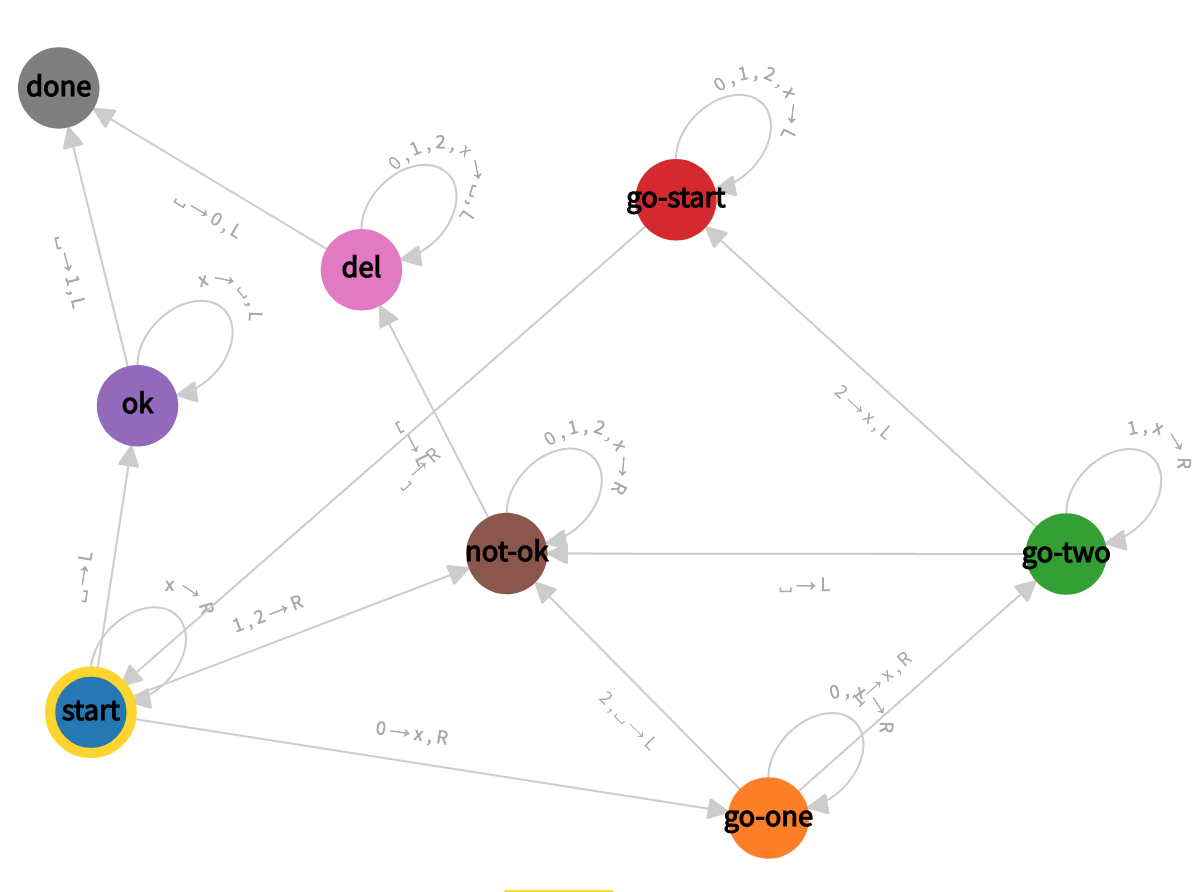
\includegraphics[width=\textwidth]{2_2_1.png} \\
        \end{center}
        
    %%%%%%%%%%%%%%%%%%%%%%%%%%%%%%%%%
    
    %%%%%%%%%%%%%%% 2 %%%%%%%%%%%%%%%
    \item Проверка соблюдения правильности скобок в строке (минимум 3 вида скобок) (0.5 балла)
    %%%%%%%%%%%%%%%%%%%%%%%%%%%%%%%%%
        Алгоритм:
        \begin{itemize}
            \item Ищем первую закрывающуюся скобку. Заменяем её на 'x'. Возвращаемся в начало.
            \item Ищем открывающуюся скобку такого же вида. Заменяем её на 'x'. Возвращаемся в начало.
            \item 1 - слов принадлежит языку (все 'x'), 0 - нет
            \item Как и в предыдущем номере, пустое слово - правильная скобочная последовательность.
        \end{itemize}
        
        \begin{minted}[]{yaml}
            # 2_2_2.yaml
            input: '([{}])'
            blank: ' '
            start state: start
            
            
            table:
              start:
                ' ': {L: ok}    # пустая скобочная послед
                ['(', '[', '{']: {R: find-closed}
                [')', ']', '}']: {L: not-ok}
                
              find-closed:
                ' ': {L: empty-or-ok}    # вышли за граицы слова или не нашли закрывающуюся скобку
                ['(', '[', '{', 'x']: R
                ')': {write: 'x', L: closed_1}
                ']': {write: 'x', L: closed_2}
                '}': {write: 'x', L: closed_3}
              
              closed_1:
                ' ': {R: not-ok}
                '(': {write: 'x', R:  find-closed}
                ['[', '{']: {L: not-ok}
                'x': L
              
              closed_2:
                ' ': {R: not-ok}
                '[': {write: 'x', R: find-closed}
                ['(', '{']: {L: not-ok}
                'x': L
            
              closed_3:
                ' ': {R: not-ok}
                '{': {write: 'x', R: find-closed}
                ['[', '(']: {L: not-ok}
                'x': L 
                
              empty-or-ok:
                ['(', '[', '{']: {L: not-ok} # всё-таки есть необработанная скобка
                'x': L
                ' ': {R: ok}
                
              not-ok:
                ['(', ')', '[', ']', '{', '}', 'x']: {write: ' ', R}
                ' ': {R: go-start}
              # в начало, чтобы очистить ленту
              go-start:
                ['(', ')', '[', ']', '{', '}', 'x']: {write: ' ', R: go-start}
                ' ': {write: 0, L: done}
                
              ok:
                ' ': {write: 1, L: done}
                'x': {write: ' ', R}
            
              done:

        \end{minted}
        \begin{center}
            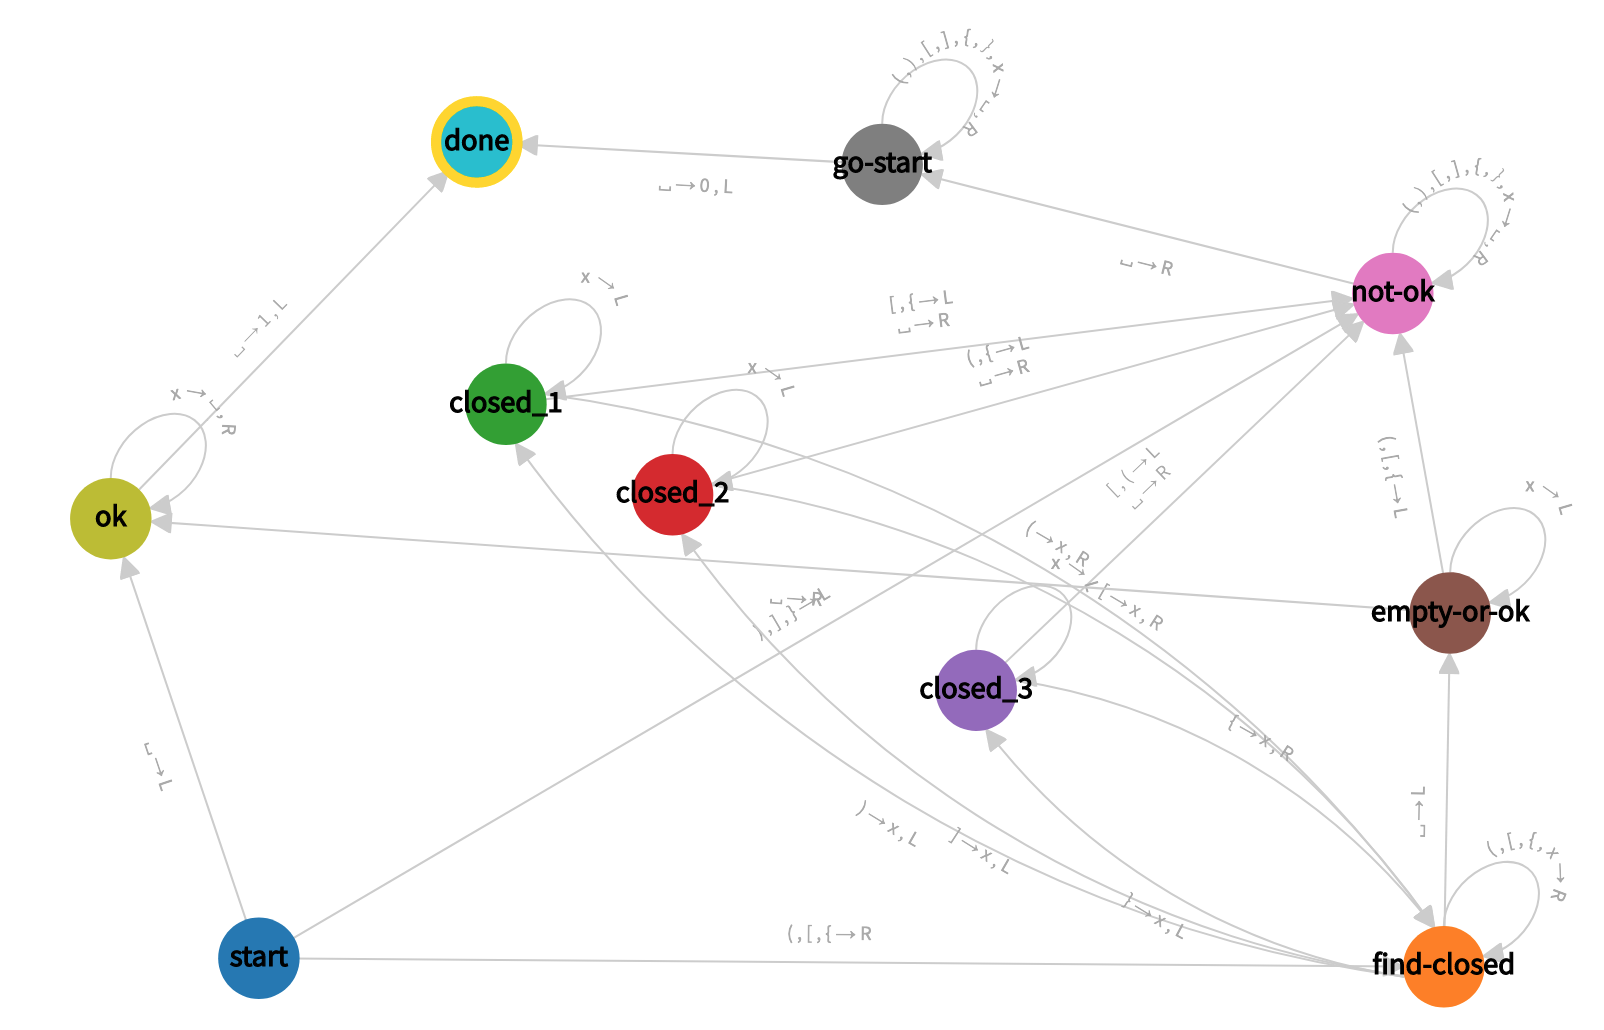
\includegraphics[width=\textwidth]{2_2_2.png} \\
        \end{center}

    %%%%%%%%%%%%%%% 3 %%%%%%%%%%%%%%%
    \item Поиск минимального по длине слова в строке (слова состоят из символов 1 и 0 и разделены пробелом) (1 балл)
    %%%%%%%%%%%%%%%%%%%%%%%%%%%%%%%%%

\section*{3 Квантовые вычисления}

\end{enumerate}
\end{document}